\documentclass[tikz,border=5pt]{standalone}
\usepackage{fontspec}
\setmainfont{Times New Roman}
\usepackage{unicode-math}
\setmathfont{Cambria Math}
\usetikzlibrary{shapes.geometric,positioning,fit,backgrounds,arrows.meta,calc}

\begin{document}
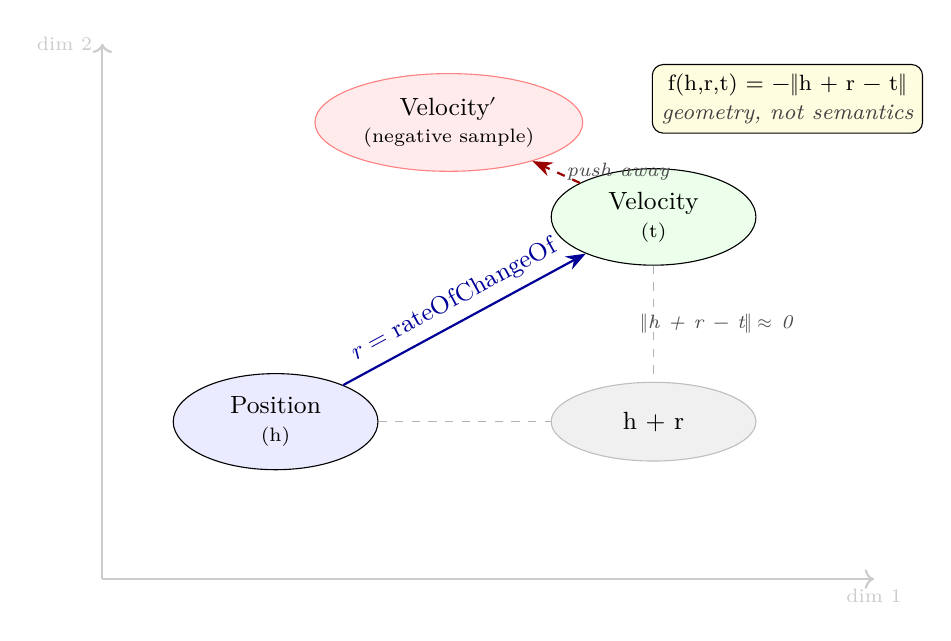
\begin{tikzpicture}[
  ent/.style={ellipse, draw, align=center, minimum width=2.6cm, minimum height=1.0cm, font=\small},
  arrow/.style={-{Stealth[length=2.5mm]}, thick},
  label/.style={font=\scriptsize\itshape, text=gray!60!black},
]

% === Embedding space axes ===
\draw[->, gray!40, thick] (-1.2, -1.2) -- (8.6, -1.2) node[below, font=\scriptsize\color{gray!60!black}] {dim 1};
\draw[->, gray!40, thick] (-1.2, -1.2) -- (-1.2, 5.6) node[left, font=\scriptsize\color{gray!60!black}] {dim 2};

% === Points ===
\node[ent, fill=blue!8] (h) at (1, 0.8) {Position\\[-1pt]\scriptsize (h)};
\node[ent, fill=green!8] (t) at (5.8, 3.4) {Velocity\\[-1pt]\scriptsize (t)};

% === Relation vector h + r ≈ t ===
\draw[arrow, blue!60!black] (h) -- (t) node[midway, above, sloped, font=\small] {$r = $ rateOfChangeOf};
\node[ent, fill=gray!12, draw=gray!50] (hr) at (5.8, 0.8) {h + r};

% === Projection lines ===
\draw[dashed, gray!60] (t) -- (hr);
\draw[dashed, gray!60] (h) -- (hr);

% === Distance label: small gap ≈ 0 ===
\node[label] at (6.6, 2.05) {$\|$h + r − t$\| \approx$ 0};

% === Corrupted negative (false negative risk) ===
\node[ent, fill=red!8, draw=red!50] (neg) at (3.2, 4.6) {Velocity$'$\\[-1pt]\scriptsize (negative sample)};
\draw[arrow, dashed, red!60!black] (t) -- node[label, right, pos=0.5] {push away} (neg);

% === Equation note ===
\node[draw, rounded corners, fill=yellow!12, align=center, font=\footnotesize] at (7.5, 4.9)
  {f(h,r,t) = −$\|$h + r − t$\|$\\[1pt] \textcolor{gray!50!black}{\itshape geometry, not semantics}};

\end{tikzpicture}
\end{document}